\documentclass{article}
\usepackage[
    paperwidth=30mm,
    paperheight=20.3mm,
    margin=0.0cm,
    noheadfoot
]{geometry}

% Required packages
\usepackage{tikz}
\usepackage{amsmath}
\usepackage{siunitx}
\usepackage{xcolor}
\usepackage{varwidth}

% TikZ libraries
\usetikzlibrary{arrows.meta,shapes.geometric,positioning,decorations.pathreplacing,calc}

% Define colors based on C2DB standards
\definecolor{sbcolor}{RGB}{159,100,181}    % Sb atoms - purple
\definecolor{tecolor}{RGB}{212,122,0}      % Te atoms - orange/gold
\definecolor{bondcolor}{RGB}{100,116,139}  % Bonds - gray
\definecolor{straincolor}{RGB}{220,38,38}  % Strain arrow - red
\definecolor{methodbox}{RGB}{240,248,255}  % Light blue for method box
\definecolor{boxblue}{RGB}{219,234,254}    % Light blue box
\definecolor{boxgreen}{RGB}{220,252,231}   % Light green box
\definecolor{boxyellow}{RGB}{254,243,199}  % Light yellow box
\definecolor{boxpink}{RGB}{252,231,243}    % Light pink box

\pagestyle{empty} % No page numbers or headers

\definecolor{Sb}{RGB}{159, 100, 181}
\definecolor{Te}{RGB}{255, 193, 37}
\tikzset{
    max width/.style args={#1}{
        execute at begin node={\begin{varwidth}{#1}},
        execute at end node={\end{varwidth}}
    }
}

\begin{document}
\begin{tikzpicture}[remember picture, overlay]

% Main title
% \node[maximum text width=\paperwidth,align=center,font=\bfseries,anchor=north,scale=0.6,xshift=-27mm,i](title) at (current page.north) {Linear optical response of monolayer Sb$_2$Te$_3$ under uniaxial strain assessed by\\ Time-Dependent Density Functional Theory};

\node[anchor=north west,xshift=1.3mm,yshift=1.2mm](str) at (current page.north west){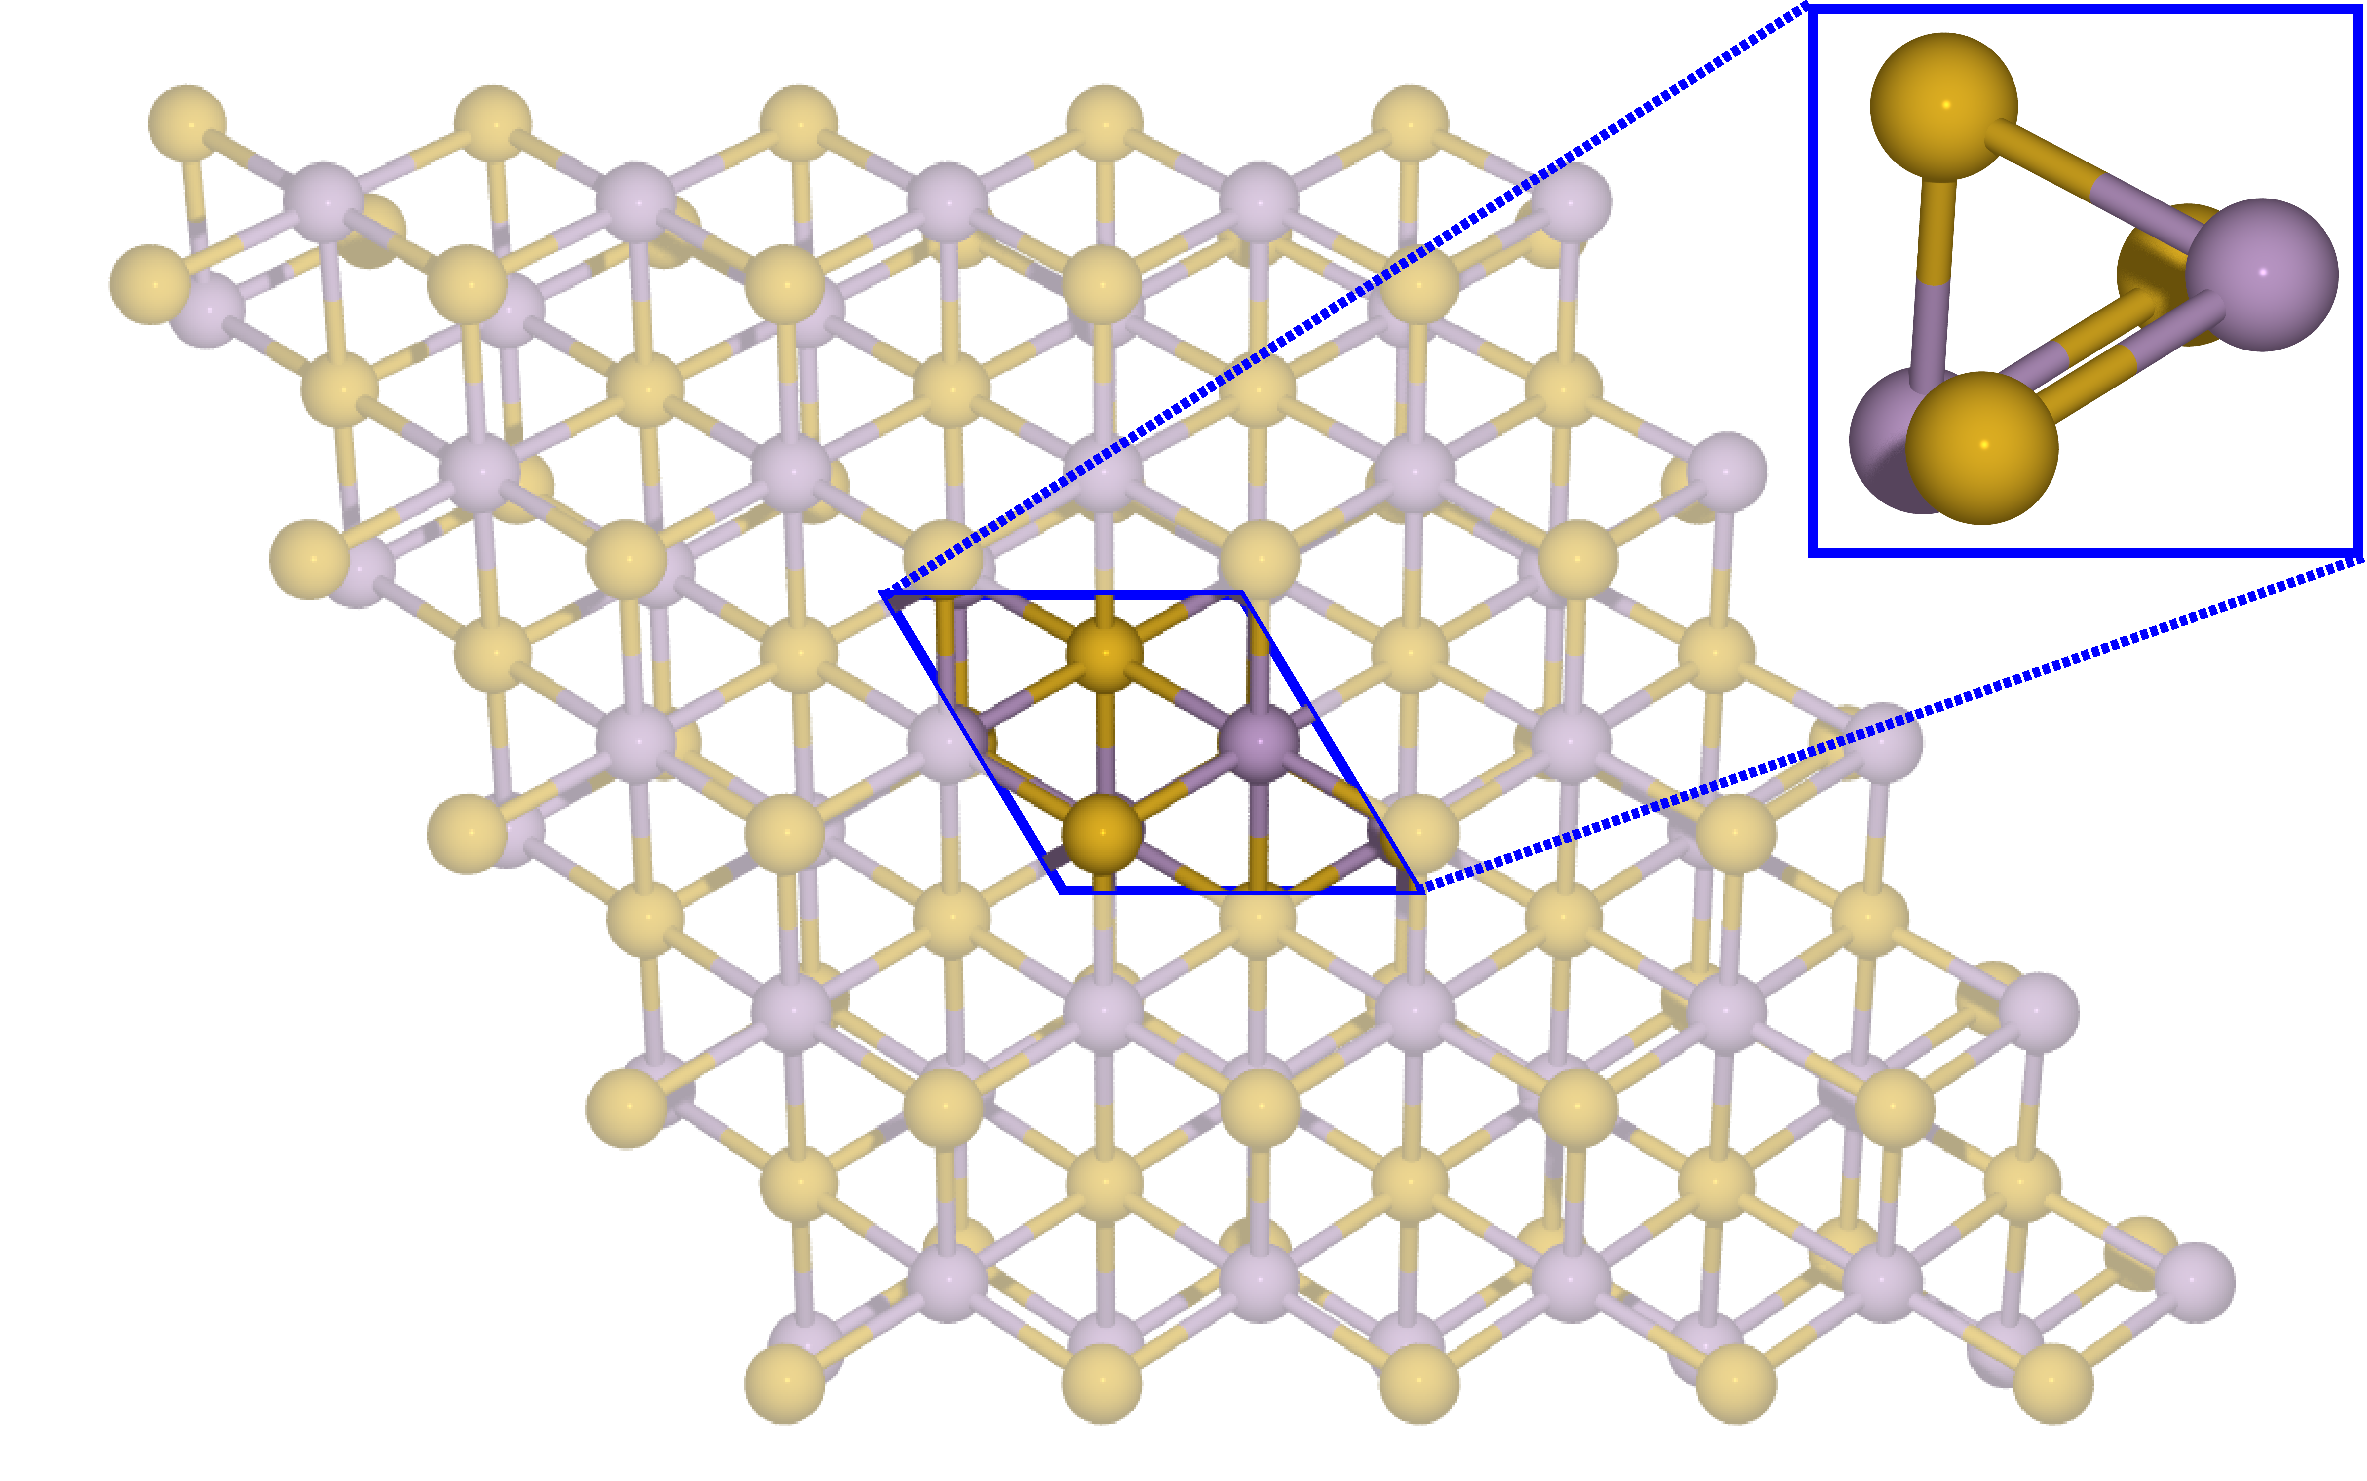
\includegraphics[width=0.9\textwidth]{build-oscar/Sb2Te3-sc.pdf}};
\node[circle,shading=ball,ball color=Sb,inner sep=0pt,outer sep=0pt,minimum size=1.5mm,xshift=5mm,yshift=-5mm] (sb) at (str.west) {};
\node[circle,shading=ball,ball color=Te,inner sep=0pt,outer sep=0pt,minimum size=1.5mm,xshift=0mm,yshift=-0.2cm] (te) at (sb.south) {};
\node[xshift=1mm,scale=0.4] at (sb.east){Sb};
\node[xshift=1mm,scale=0.4] at (te.east){Te};

\node[anchor=north,red, text width=5cm,scale=0.4,xshift=5mm,align=center](l1) at (str.south){Uniaxial Strain $+x$ (0-5\%) };
\draw[-{Stealth},red] ([shift={(10mm,1mm)}]str.south west)--([shift={(-5mm,1mm)}]str.south east);

\draw[-{stealth},line width=0.25mm,inner sep=0mm,red]([xshift=-0.5mm,yshift=-10mm]str.north west)--++(4mm,0cm) node[black,scale=0.4,xshift=1.3mm] {$x$};
\draw[-{stealth},line width=0.25mm,inner sep=0mm,green!90!black]([xshift=-0.5mm,yshift=-10mm]str.north west)--++(0cm,4mm) node[black,scale=0.4,yshift=1.5mm] {$y$};
\filldraw[blue] ([xshift=-0.5mm,yshift=-10mm]str.north west) circle (1pt);

% \begin{scope}[scale=0.1]
% \draw[-{stealth},line width=0.75mm,inner sep=0mm,red]([xshift=3mm,yshift=-8mm]str.north west)--++(1.0cm,0cm);
% \draw[-{stealth},line width=0.75mm,inner sep=0mm,green!90!black]([xshift=3mm,yshift=-8mm]str.north west)--++(0cm,1.0cm);
% \filldraw[blue] ([xshift=3mm,yshift=-8mm]str.north west) circle (3pt);
% \node at ([xshift=14mm,yshift=-8mm]str.north west){$x$};
% \node at ([xshift=3mm,yshift=4mm]str.north west){$y$};        
% \end{scope}

\end{tikzpicture}

\end{document}